\documentclass[hyperref={pdfpagelabels=false}]{beamer}
\usepackage{lmodern}
\usetheme{CambridgeUS}

\title{\\Portale per la visualizzazione di gene expression\\}  
\author{\\ C. Bartalotta, D. Santilli e D. Bernardini} 
\date{\today} 
\begin{document}
\logo{
\includegraphics[scale=0.04]{logoMendel}}
\begin{frame}
\titlepage
\end{frame} 

\begin{frame}\frametitle{Problema}
\textbf{Espressione genica:}\\
processo grazie al quale l'informazione contenuta in un gene viene convertita in una macromolecola funzionale.
\'E un processo a pi\'u stadi:\pause 
\begin{enumerate}
\item trascrizione del DNA in RNA:\\
produzione dell'RNA complementare a una delle due eliche del gene  \pause 
\item maturazione:\\
l'RNA trascritto puo' essere modificato (maturazione) per dare origine a quello che si chiama RNA (funzionante) maturo \pause 
\item traduzione:\\
l'RNA messaggero o mRNA viene tradotto nella proteina corrispondente
\end{enumerate}
\textbf{Analisi di Espressione Differenziale:}\\
Processo statistico usualmente impiegato per identificare i geni che sono espressi in maniera differenziale fra due gruppi a confronto.\\
\end{frame}

\begin{frame}\frametitle{Obiettivi}
\begin{itemize}
\item Possibilit\'a di gestire esperimenti composti da pi\'u analisi di espressione differenziale eseguiti su circa 30.000 geni diversi
\item Acquisire informazioni per ogni singolo gene ottenuto tramite querying dell'utente
\item Possibilit\'a di visualizzare analisi composte dai soli campi d'interesse per l'utente
\end{itemize}
\end{frame}

\begin{frame}\frametitle{Servizi per l'utente}
\begin{block}{Super-user}
\begin{itemize}
\item creare/modificare/cancellare esperimenti
\item inserire una o pi\'u analisi differenziali per ogni esperimento
\item autorizzare uno o pi\'u utenti a poter visualizzare uno o pi\'u esperimenti
\end{itemize}
\end{block}
\begin{exampleblock}{User}
\begin{itemize}
\item scegliere quale analisi di un esperimento visualizzare
\item filtrare solo determinati geni o determinati valori di p-value e fold-change
\end{itemize}
\end{exampleblock}
\bigskip
\bigskip
\bigskip
\end{frame}

\begin{frame}\frametitle{Struttura dati}

Struttura di un esperimento: \bigskip

\resizebox{\textwidth}{!}{%
\begin{tabular}{|c|c|c|c|c|c|c|}
\hline
\textbf{Gene} & \textbf{...} & \textbf{p-value(A)} & \textbf{Fold-change(A)} & \textbf{...} & \textbf{p-value(B)} & \textbf{Fold-change(B)} \\
\hline
BST2 & \textbf{...} & 0.434208 & 1.50149 & \textbf{...} & 7.54353e-010 & 142.989  \\
\hline
SAMD9L & \textbf{...} & 0.530237 & -1.4498 & \textbf{...} & 2.19109e-008 & 123.924 \\
\hline
\textbf{...} & \textbf{...} & \textbf{...} & \textbf{...} & \textbf{...} & \textbf{...} & \textbf{...} \\
\hline
\end{tabular}}
\bigskip

Ogni esperimento \'e composto da pi\'u analisi (nell'esempio A e B).\\
I dati di ogni analisi sono rappresentati attraverso pi\'u colonne.\\
\bigskip
Fold change = misura la variazione del livello di espressione di un gene, da un valore iniziale ad uno finale\\
\bigskip
p-value = probabilit\'a di ottenere un risultato pari o pi\'u estremo di quello osservato (Se il p-value \'e minore di una certa soglia allora una serie di dati sar\'a statisticamente significativa)


\end{frame}

\begin{frame}\frametitle{Analisi e progettazione}
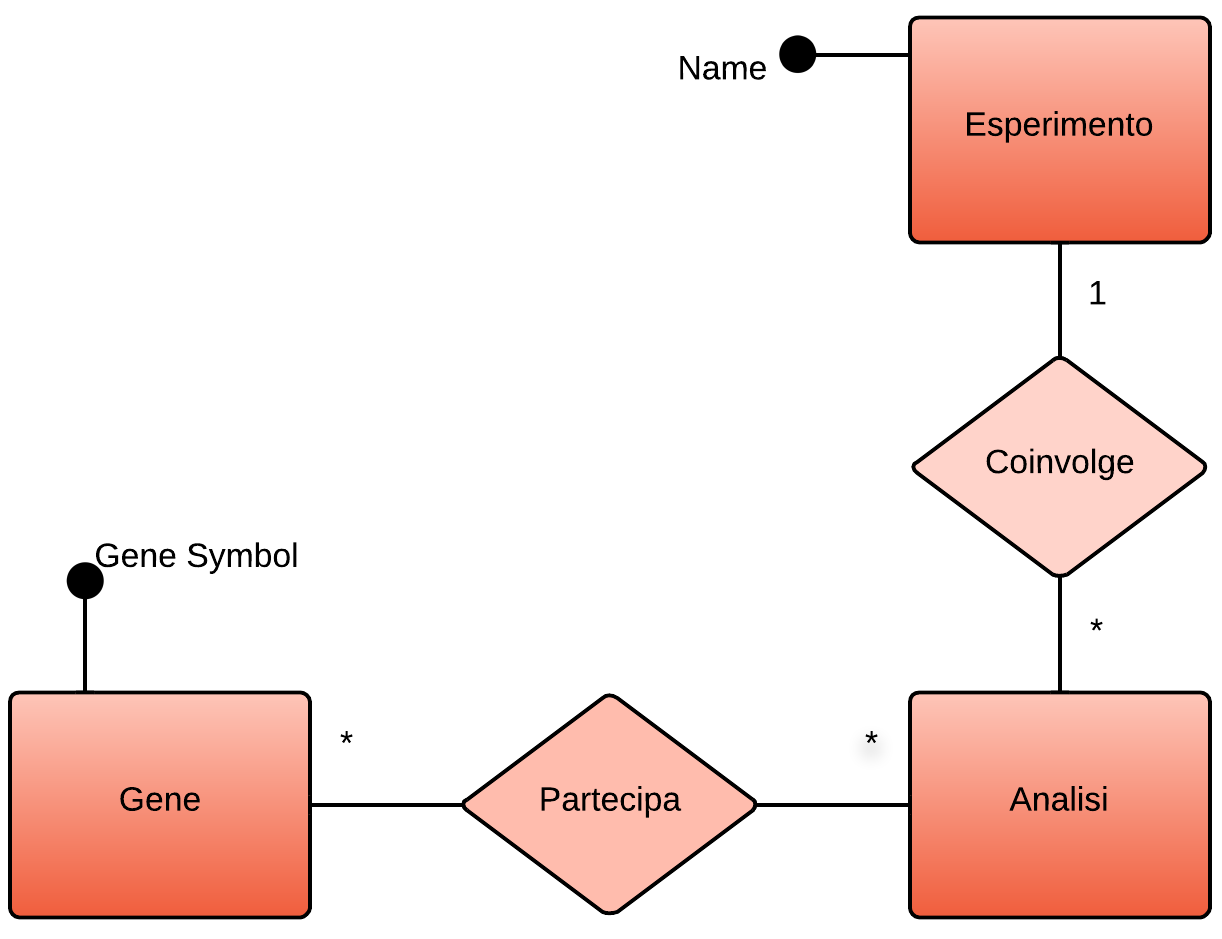
\includegraphics[width=10cm,height=6.75cm]{er.png}
\end{frame}

\begin{frame}\frametitle{Analisi e progettazione}
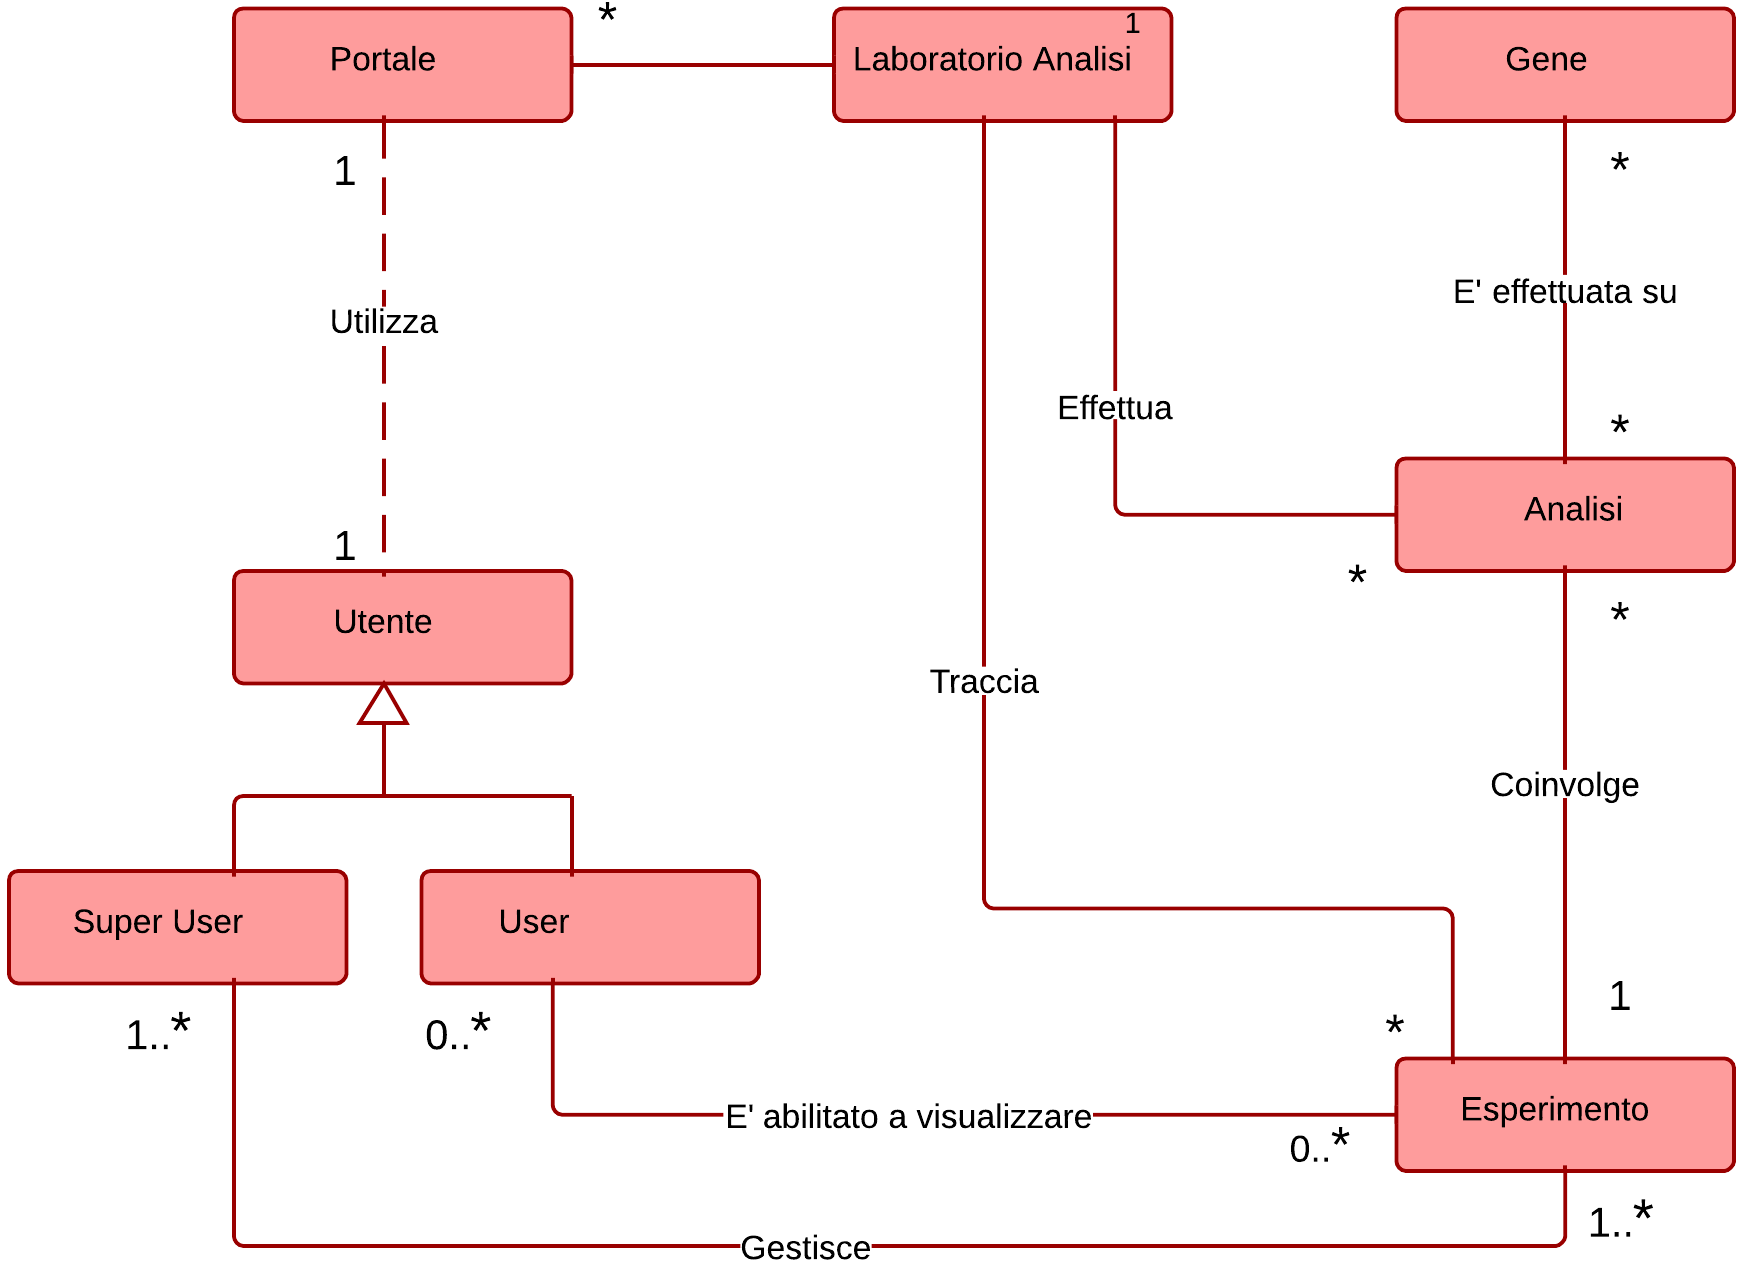
\includegraphics[width=10cm,height=6.75cm]{uml.png}
\end{frame}

\begin{frame}\frametitle{Tecnologie}
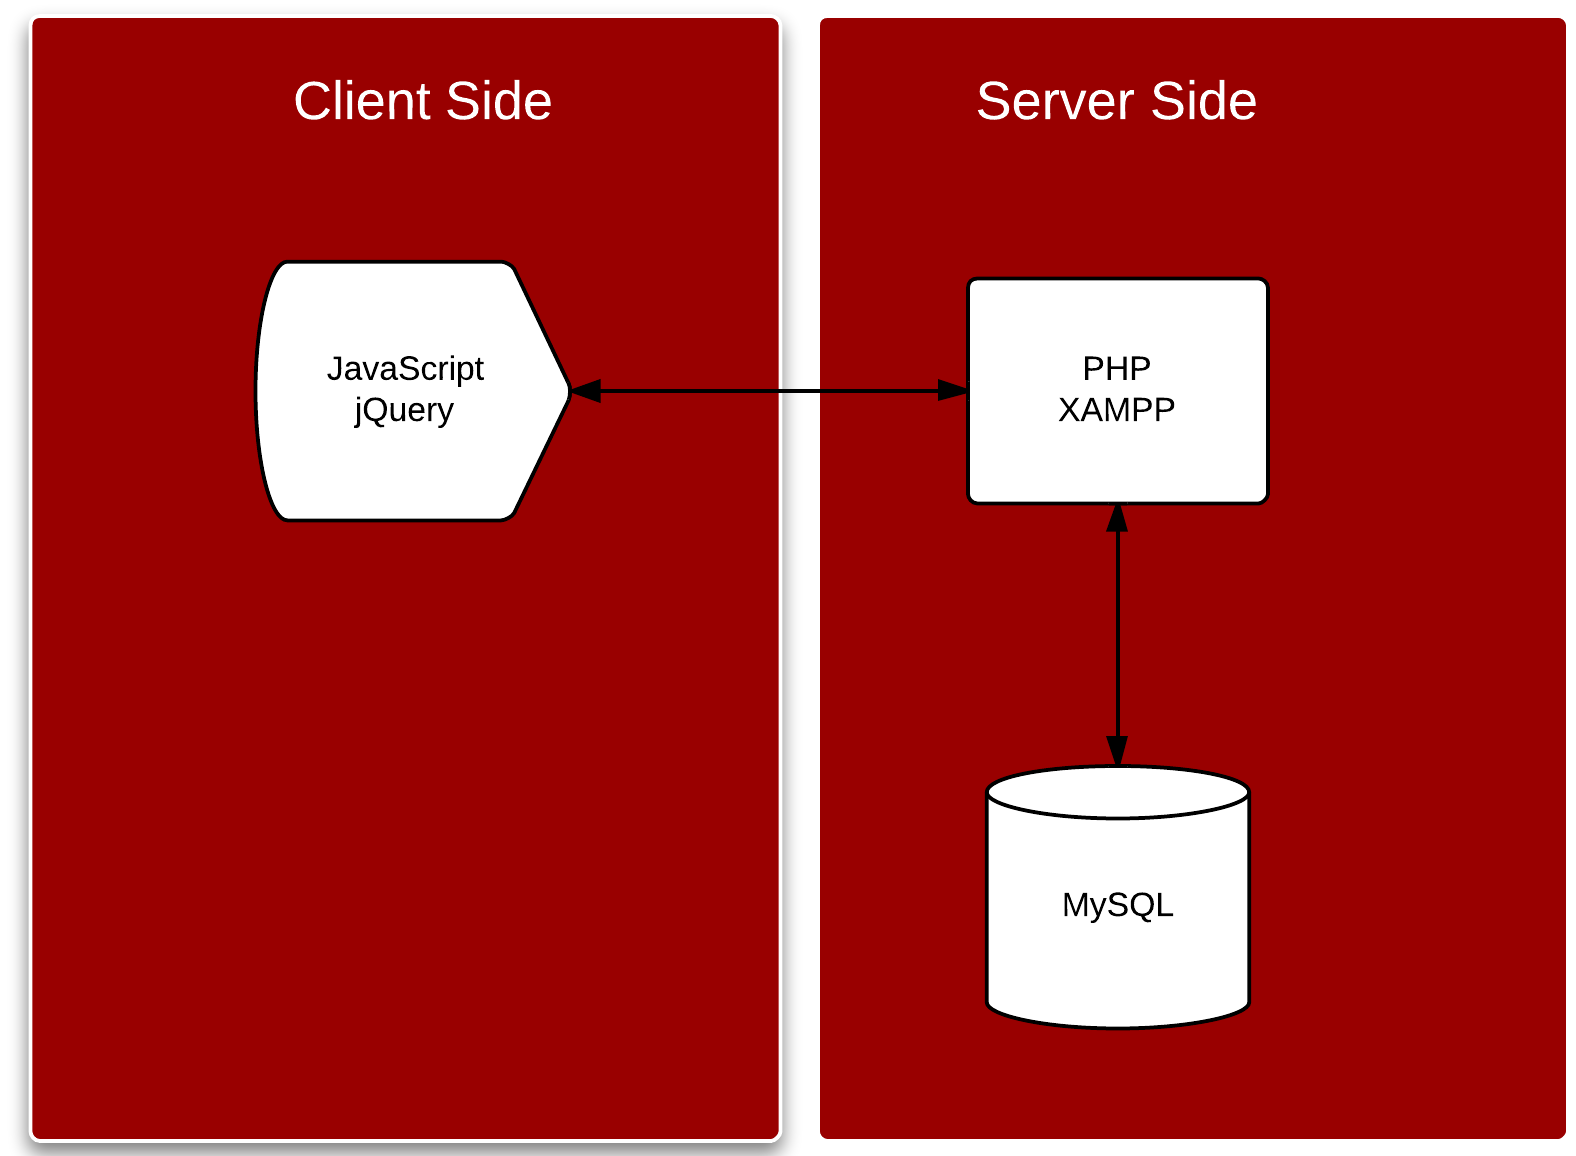
\includegraphics[width=11.25cm,height=7cm]{tecnologie.png}
\end{frame}

\begin{frame}\frametitle{XAMPP}
\begin{minipage}[c]{.4\textwidth}
	
\includegraphics[width=4.5cm,height=4.5cm]{xampp.png}
\end{minipage}%
\
\begin{minipage}[c]{.55\textwidth}
	XAMPP \'e una piattaforma software gratuita costituita da Apache HTTP Server, il database MySQL e tutti gli strumenti necessari per utilizzare il linguaggio di programmazione PHP;\\
	attraverso l'utilizzo di XAMPP \'e possibile quindi avere un application server capace di interpretare pagine web PHP dinamiche.
\end{minipage}
\end{frame}

\begin{frame}\frametitle{Divisione del lavoro}
\begin{itemize}
\item Chiara Bartalotta: \textcolor{blue}{front-end}, \textcolor{green}{back-end}
\item Dario Santilli: \textcolor{blue}{front-end}, \textcolor{red}{database}
\item Davide Bernardini:  \textcolor{red}{database}, \textcolor{green}{back-end}
\end{itemize}
\end{frame}

\end{document}

